\subsection{Addestramento}


Da quanto detto nel paragrafo precedente, \emph{si ricorre ad una rete neurale} 
per approssimare la media e la varianza delle transizioni~\eqref{eq:reverse_transition} intrattabili della diffusione inversa.


\noindent Nella scelta della funzione di costo da minimizzare per allenare la rete neurale, la \emph{ratio} perseguita è la seguente.
Dal momento che si possono ravvisare delle affinità tra il processo di diffusione inversa e il 
decoder di un \emph{autoencoder variazionale} (VAE) (si veda~\ref{fig:VAE_vs_Diff}), è 
legittimo avvalersi della medesima funzione di costo usata nei VAE: 
il logaritmo della funzione di verosimiglianza cambiato di segno (\emph{Negative Log-Likelihood})(\ref{ssec:verosimiglianza}).
Pertanto, la funzione di costo da minimizzare è:
\begin{equation}
 L=-\log\bigl(p_{\bm{\theta}}(\mathbf{x}_0)\bigr)
\end{equation}
Tuttavia, esplicitando la funzione di verosimiglianza $p_{\bm{\theta}}(\mathbf{x}_0)$
\begin{equation}
 p_{\bm{\theta}}(\mathbf{x}_0)=\int p_{\bm{\theta}}(\mathbf{x}_{0:T}) \,d\mathbf{x}_{1:T} \label{eq:intractable_likelihood}
\end{equation}
si desume che $p_{\bm{\theta}}(\mathbf{x}_0)$ (e quindi $L$) è \emph{intrattabile}, essendo 
l'integrale nella~\eqref{eq:intractable_likelihood} esteso ad uno spazio (di pixel) ad alta dimensionalità.
Si ricorre, quindi, al tipico \emph{pattern} di approssimare una funzione intrattabile con un suo \emph{lower bound} 
(Figura~\ref{fig:vlb}) che ammetta, invece, un'espressione in forma chiusa.
\begin{figure}
    \centering
    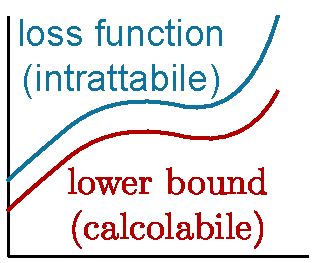
\includegraphics[keepaspectratio, scale=0.5]{lower_bound.pdf}
    \caption{\emph{Lower bound} di una funzione. Fonte~\cite{royBeginnerGuideDiffusion}.} 
    \label{fig:vlb}
\end{figure}
Invocando, ancora una volta, l'affinità intercorrente tra il processo di diffusione inversa e il decoder 
di un VAE, si può ricorrere al \emph{lower bound variazionale} (VLB) (o \emph{lower bound dell'evidenza} (ELBO)) che, 
declinato al contesto dei modelli di diffusione, è:
\begin{equation}
    \log \bigl(p_{\bm{\theta}}(\mathbf{x}_0)\bigr)\geq\underbrace{\mathbb{E}_q\biggl[\log\frac{p_{\bm{\theta}}(\mathbf{x}_{0:T})}{q(\mathbf{x}_{1:T}|\mathbf{x}_0)}\biggr]}_{VLB}
\end{equation}
(si veda Appendice~\ref{appendix:details_loss} per la derivazione dettagliata), e, come si vedrà nel prosieguo, risulterà essere trattabile. 
Pertanto, minimizzare la funzione di costo $L$ significa minimizzare il VLB cambiato di segno:
\begin{equation}
    L=-\log \bigl(p_{\bm{\theta}}(\mathbf{x}_0)\bigr)\leq L_{vlb}\triangleq\mathbb{E}_q\biggl[-\log\frac{p_{\bm{\theta}}(\mathbf{x}_{0:T})}{q(\mathbf{x}_{1:T}|\mathbf{x}_0)}\biggr]
\end{equation}
\begin{oss}
A rigore l'uso del pedice \emph{vlb} in $L_{vlb}$ è un abuso di notazione, dal momento che $L_{vlb}$ non è 
un lower bound ma è un \emph{upper bound} della funzione di costo $L$. Tuttavia, si predilige 
tale notazione $L_{vlb}$ per essere consistenti con la letteratura.
\end{oss}
\noindent A valle di una serie di calcoli che sono riportati in Appendice~\ref{appendix:details_loss} si perviene al seguente risultato:
\begin{equation}
    L_{vlb}=L_0+\sum_{t=2}^TL_{t-1}+L_T \label{eq:Lvlb}
\end{equation}
dove:
\begin{itemize}
    \item $L_0=-\log \bigl(p_{\bm{\theta}}(\mathbf{x}_0|\mathbf{x}_1)\bigr)$. Ho et al.~\cite{ho2020} hanno delegato ad un apposito decoder l'approssimazione di tale termine
    che, pertanto, può essere trascurato nella fase di addestramento della rete neurale.
    \item $L_{t-1}=D_{KL}\bigl(q(\mathbf{x}_{t-1}|\mathbf{x}_t,\mathbf{x}_0)\,\|\,p_{\bm{\theta}}(\mathbf{x}_{t-1}|\mathbf{x}_t)\bigr)$. L'obiettivo  
    è quello di addestrare la rete neurale, cosicché $p_{\bm{\theta}}(\mathbf{x}_{t-1}|\mathbf{x}_t)$ approssimi 
    quanto più fedelmente la distribuzione $q(\mathbf{x}_{t-1}|\mathbf{x}_t,\mathbf{x}_0)$ in 
    modo da minimizzare il termine $L_{t-1}$ (ricorrendo all'usuale interpretazione della \emph{divergenza di Kullback-Leibler} 
    (Appendice~\ref{appendix:details_loss},~\ref{eq:kullback-leibler})
    come una misura della distanza tra le distribuzioni).
    \item $L_T=D_{KL}\bigl(q(\mathbf{x}_T|\mathbf{x}_0)\,\|\,p(\mathbf{x}_T)\bigr)$ è un termine che può essere \emph{ignorato} durante 
    la fase di addestramento, dal momento che non annovera alcun parametro che possa essere appreso dalla rete neurale. 
    Infatti $p(\mathbf{x}_T)=q(\mathbf{x}_T)\sim\mathcal{N}(\bm{0},\bm{I})$ 
    e $q(\mathbf{x}_T|\mathbf{x}_0)$ è fissato una volta scelti gli iperparametri $\beta_t$~\eqref{eq:forward_diff_v2}.
\end{itemize}

\begin{oss}
    Definendo uno schema di diffusione opportuno (i.e.\ i valori dei $\beta_t$)
    e scegliendo l'iperparametro $T$ sufficientemente elevato, entrambe le distribuzioni 
    $q(\mathbf{x}_T|\mathbf{x}_0)$ e $p(\mathbf{x}_T)$ approssimano una gaussiana standard. 
    Quindi, stante l'interpretazione della divergenza di Kullback-Leibler come una misura della distanza tra tali distribuzioni,
    il termine $L_T=D_{KL}\bigl(q(\mathbf{x}_T|\mathbf{x}_0)\,\|\,p(\mathbf{x}_T)\bigr)$ tende a zero.
\end{oss}
\noindent Dunque, affinché $L_{vlb}$ risulti trattabile è sufficiente che $L_{t-1}$ ammetta un'espressione in forma chiusa.

\noindent Restringendo l'attenzione al termine $L_{t-1}$, 
in Appendice~\ref{sec:detailed_loss_term} si mostra che sussistono le seguenti considerazoni:
\begin{itemize}
\item poiché:
\begin{align}
    q(\mathbf{x}_{t-1}|\mathbf{x}_t,\mathbf{x}_0) &= \mathcal{N}(\mathbf{x}_{t-1}; \tilde{\bm{\mu}}_{t}(\mathbf{x}_t,\mathbf{x}_0),\tilde{\beta_t} \bm{I}) \label{eq:rif1}\\
    p_{\theta}(\mathbf{x}_{t-1}|\mathbf{x}_t)&=\mathcal{N}(\mathbf{x}_{t-1};\bm{\mu}_{\bm{\theta}}(\mathbf{x}_t,t),\bm{\Sigma}_{\bm{\theta}}(\mathbf{x}_t,t)) \label{eq:rif2}
\end{align}
segue che $L_{t-1}=D_{KL}\bigl(q(\mathbf{x}_{t-1}|\mathbf{x}_t,\mathbf{x}_0)\,\|\,p_{\theta}(\mathbf{x}_{t-1}|\mathbf{x}_t)\bigr)$ è 
la divergenza di Kullback-Leibler tra due gaussiane, e in quanto tale può essere espresso in forma chiusa. 
\item nella~\eqref{eq:rif2}, sebbene in linea di principio si possa addestrare 
la rete neurale ad apprendere sia $\bm{\mu}_{\bm{\theta}}(\mathbf{x}_t,t)$ che $\bm{\Sigma}_{\bm{\theta}}(\mathbf{x}_t,t)$, Ho et al.~\cite{ho2020} 
hanno \emph{fissato la varianza}  $\bm{\Sigma}_{\bm{\theta}}(\mathbf{x}_t,t)=\beta_t\bm{I}$. Quindi nella fase di addestramento 
la rete neurale deve apprendere la sola media $\bm{\mu}_{\bm{\theta}}(\mathbf{x}_t,t)$.
\item anziché addestrare la rete neurale ad apprendere, in ogni passo di diffusione inversa, la media $\bm{\mu}_{\bm{\theta}}(\mathbf{x}_t,t)$, 
si mostra che la rete può equivalentemente essere addestrata a predire il rumore $\bm{\epsilon}_{\bm{\theta}}(\mathbf{x}_t,t)$
che deve essere rimosso in ogni step della diffusione inversa per giungere all'immagine di partenza.
\end{itemize}

\noindent Stante i suddetti risultati, in Appendice~\ref{appendix:details_loss} si mostra che ognuno degli $L_{t-1}$ nella~\eqref{eq:Lvlb} 
assume la seguente forma semplificata:
\begin{equation}
    L_{t-1}^{\text{simple}}=\Vert \bm{\epsilon}-
    \bm{\epsilon}_{\bm{\theta}}(\underbrace{\sqrt{\overline{\alpha}_t}\mathbf{x}_0+\sqrt{1-\overline{\alpha}_t}\bm{\epsilon}}_{\mathbf{x}_t},t)\Vert^2 +C
    \label{eq:simple_loss}
\end{equation}
dove $C$ è una costante che non dipende da $\bm{\theta}$ e, quindi, può essere ignorata durante l'addestramento.

In definitiva, partendo da una funzione di costo $L=-\log\bigl(p_{\bm{\theta}}(\mathbf{x}_0)\bigr)$ intrattabile 
si è giunti alla~\eqref{eq:simple_loss}, in cui ognungo degli $L_{t-1}$ è, banalmente, l'\emph{errore quadratico medio} tra il rumore $\bm{\epsilon}$, aggiunto nella diffusione in avanti, e 
il rumore \emph{stimato} della rete neurale $\bm{\epsilon}_{\bm{\theta}}(\mathbf{x}_t,t)$.


\subsubsection{Architettura della rete neurale e algoritmo di addestramento}
Dal momento che la rete neurale deve fornire in uscita un'immagine (i.e.\ la stima del rumore), 
che è un \emph{tensore} avente le stesse dimensioni dell'immagine rumorosa in ingresso alla rete, 
Ho et al.~\cite{ho2020} hanno implementato la suddetta rete neurale con una U-Net, in virtù della sua peculiarità di produrre un'immagine 
con le medesime dimensioni dell'immagine in ingresso.
In Appendice~\ref{appendix:unet} sono riportati ulteriori dettagli sulla U-Net utilizzata in un DDPM.
\begin{algorithm}[H]
    \caption{Addestramento. Fonte~\cite{ho2020}}\label{alg:training}
   \begin{algorithmic}[1]
    \Repeat    
   \State $\mathbf{x}_0 \sim q(\mathbf{x}_0)$\label{row:training1}
    \State $t \sim \text{Uniform$(\{2,...,T\})$}$\label{row:training2}
   \State $\boldsymbol{\epsilon}\sim \mathcal{N}(\bm{0},\bm{I})$\label{row:training3}
   \State $\mathbf{x}_t=\sqrt{\overline{\alpha}_t}\mathbf{x}_0+\sqrt{1-\overline{\alpha}_t}\bm{\epsilon}$\label{row:training4}
   \State Take gradient descent step on
    \State $\qquad \nabla_{\bm{\theta}} \Vert \bm{\epsilon}-\bm{\epsilon_{\theta}}(\mathbf{x}_t,t) \Vert^2$\label{row:training5}
    \Until converged
   \end{algorithmic}
\end{algorithm}
\noindent In Figura~\ref{fig:training} è illustrato il meccanismo sotteso ad un passo dell'algoritmo di addestramento (Algoritmo~\ref{alg:training}) 
della rete neurale. Nell'Algoritmo~\ref{alg:training}:
\begin{figure}
    \centering
    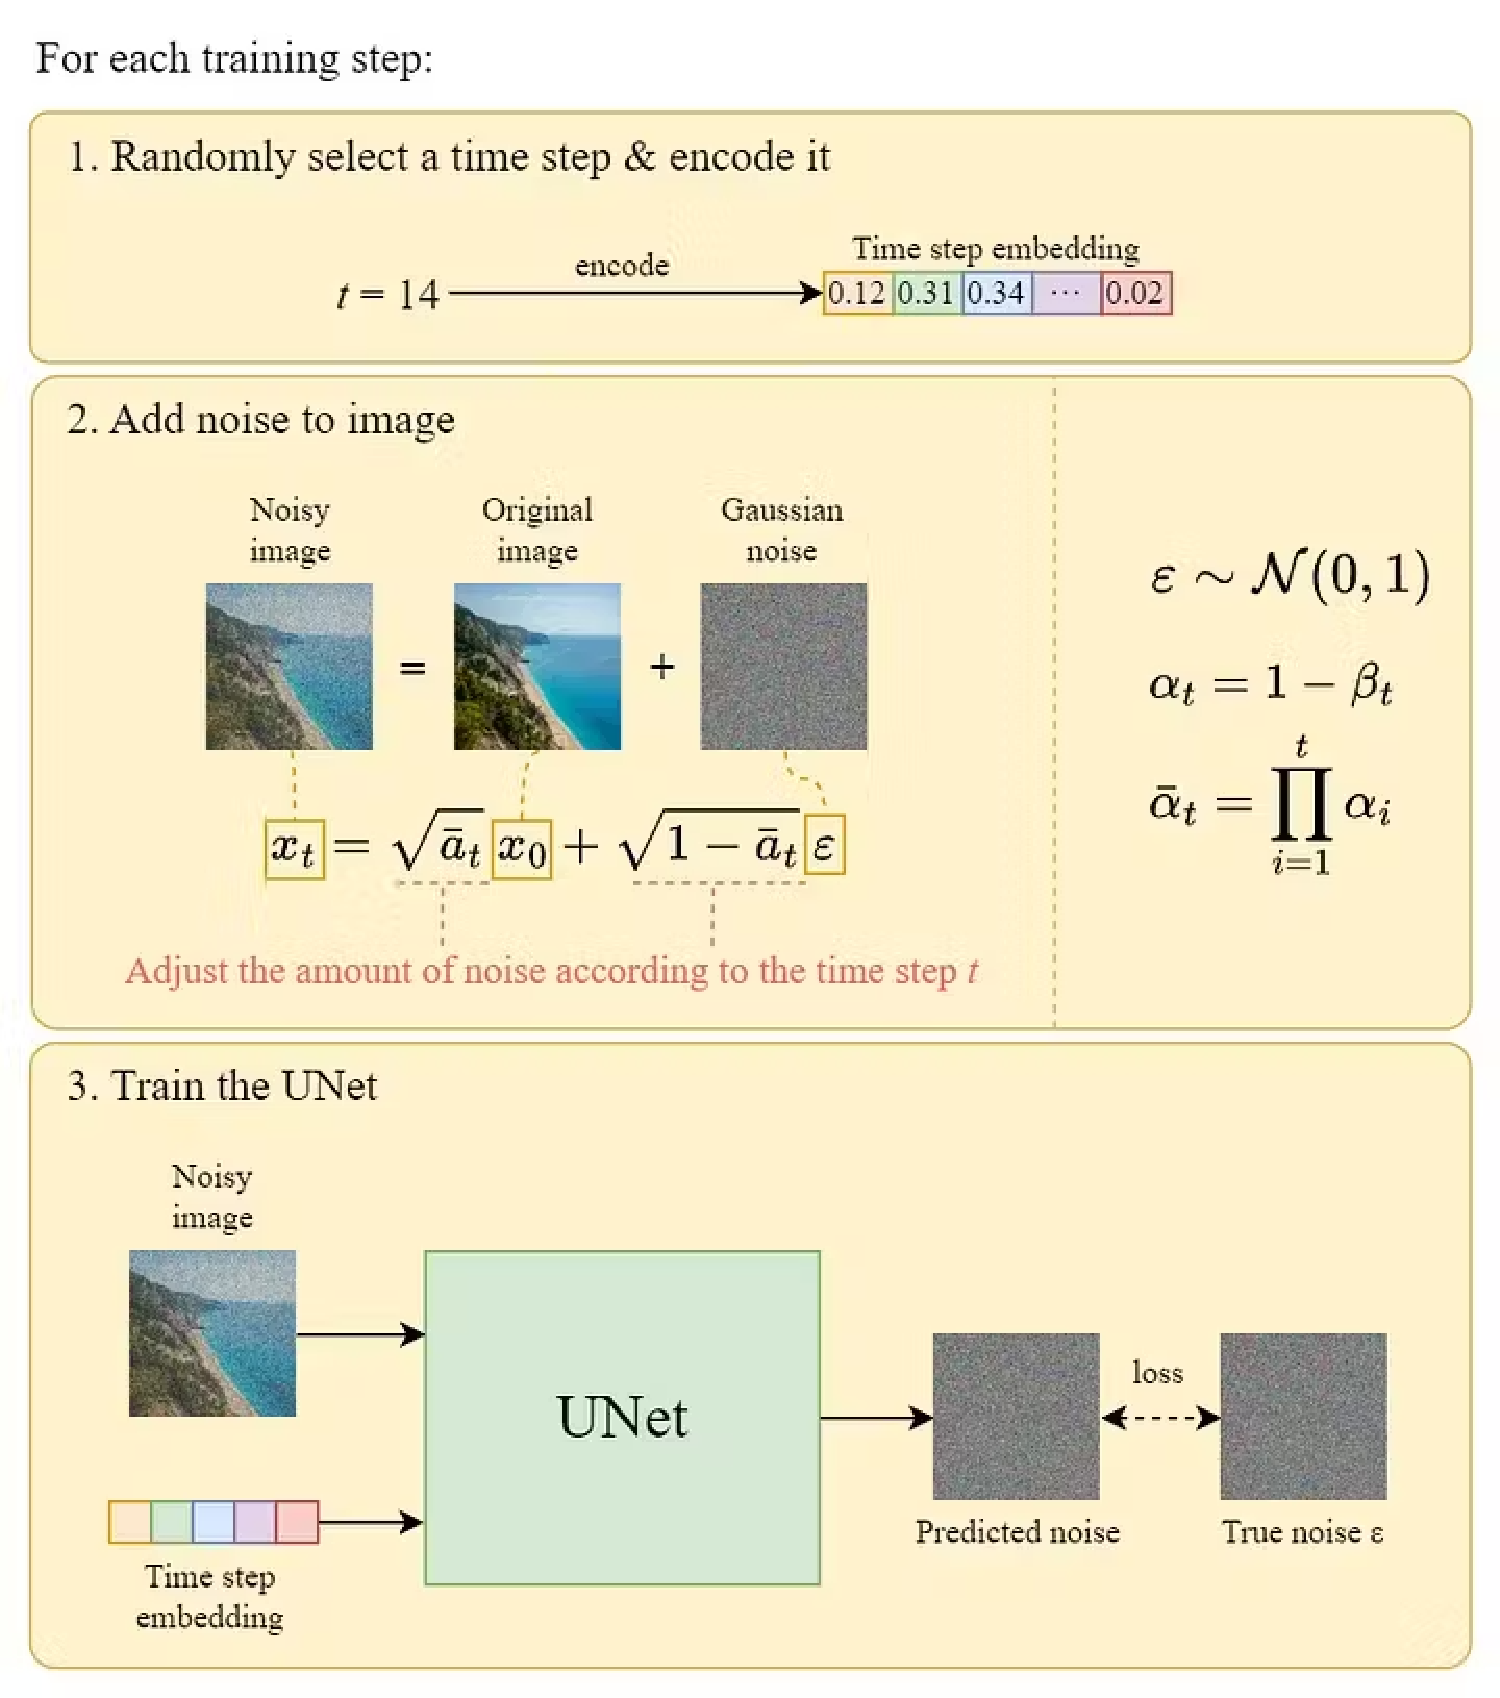
\includegraphics[keepaspectratio, scale=0.45]{training.pdf}
    \caption{Addestramento della rete neurale. Fonte~\cite{royBeginnerGuideDiffusion}.}
    \label{fig:training}
\end{figure}

\begin{itemize}
\item si considera un'immagine $\mathbf{x}_0$, nel dataset di addestramento, caratterizzata da una distribuzione incognita e arbitrariamente complessa $q(\mathbf{x}_0)$ (riga~\ref{row:training1}).
\item si seleziona \emph{a caso} (ciò giustifica il ricorso alla distribuzione uniforme) un passo temporale $t$ (riga~\ref{row:training2}).
\item si campiona del rumore $\bm{\epsilon}$ da una gaussiana standard (riga~\ref{row:training3}).
\item si applica il processo di diffusione in avanti nella sua versione ottimizzata~\eqref{eq:eff_forward}, per ottenere l'immagine rumorosa 
$\mathbf{x}_t$ a partire da $\mathbf{x}_0$ (riga~\ref{row:training4}).
\item si minimizzano i termini $L_{t-1}^{\text{simple}}=\Vert \bm{\epsilon}-\bm{\epsilon_{\theta}}(\mathbf{x}_t,t)\Vert^2$ 
con la tecnica del gradiente discendente stocastico (riga~\ref{row:training5}).
\end{itemize}

\begin{oss}
    Si noti come la riformulazione~\eqref{eq:eff_forward}  del processo di diffusione in avanti 
    permetta di scegliere \emph{a caso} il passo temporale $t$, e quindi il termine $L_{t-1}$ da ottimizzare, con il gradiente discendente, nella fase di 
    addestramento. 
\end{oss}









